 
\section{DenseBox for Detection }
\label{sec:model} 
	\begin{figure}[!hbtp]
	\centering
	 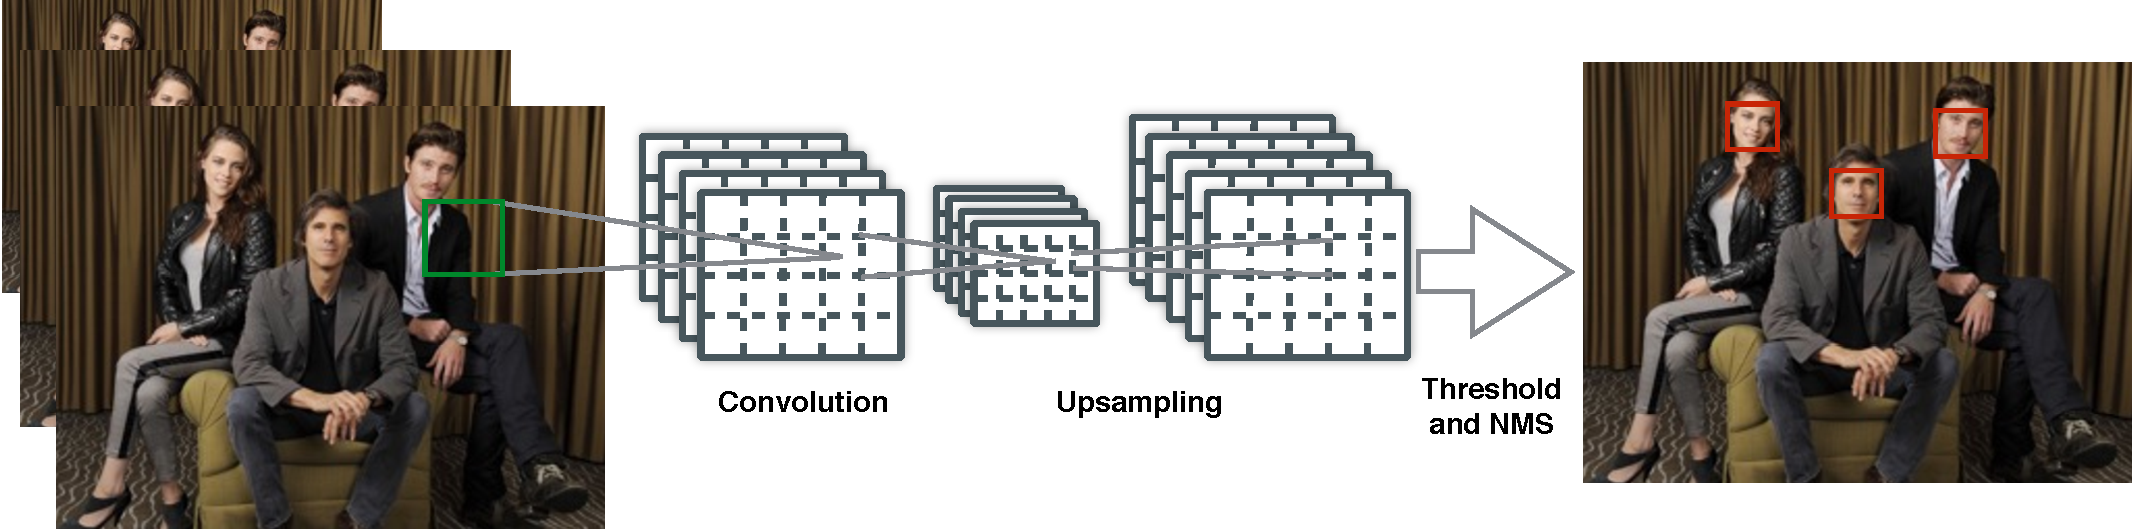
\includegraphics[scale=0.39]{figures/figure1-crop.pdf}
	\caption{\textbf{The DenseBox Detection Pipeline.} 1) Image pyramid is fed to the network. 2) After several layers of convolution and pooling, upsampling feature map back and apply convolution layers to get final output. 3) Convert output feature map to bounding boxes , and apply non-maximum suppression to all bounding boxes over the threshold. }
	\label{fig:fig_overview}
	\end{figure}


The whole detection system is illustrated in Fig \ref{fig:fig_overview}. The single convolutional network simultaneously output multiple predicted bounding boxes and class confidence. All components of object detection in R-CNN are modeled as a fully convolutional network except the non-maximum suppression step, so region proposal generation is unnecessary. In the test, the system takes an image (at the size of $m\times n$) as input, and output a $ \frac{m}{4} \times \frac{n}{4} $ feature map with 5 channels.
If we define the left top and right bottom points of the target bounding box in output coordinate space as $ p_t = (x_t, y_t)$ and as $ p_b = (x_b, y_b)$ respectively, then each pixel $i$ located at $(x_i, y_i)$ in the output feature map describe a bounding box with a 5-dimensional vector $\hat{t_i } = \{ \hat{s }, \hat{dx^{t}= x_i - x_t,},\hat{dy^{t}} = y_i - y_t,\hat{dx^{b}}= x_i - x_b,\hat{dy^{b}}= y_i - y_b \}_i$ , where $\hat{s }$ is the confidence score of being an object and $\hat{dx^{t}}$, $\hat{dy^{t}}$,$\hat{dx^{b}}$, $\hat{dy^{b}}$ denote the distance between output pixel location with the boundary of target bounding box. Finally every pixel in the output map is converted to bounding box with score, and non-maximum suppression is applied to those boxes whose scores pass the threshold. 

\subsection{Ground Truth Generation } 

It is unnecessary to put the whole image into the network for training because it would take most computation time in convolving on background. A wise strategy is to crop large patches containing faces and sufficient background information for training. In this paper, we train our network on single scale, and apply it to multiple scales for evaluation. 

Generally speaking, our proposed network is trained in a segmentation-like way.   In training, the patches are cropped and resized to $240 \times 240$ with a face in the center roughly has the height of 50 pixels. The output ground truth in training is a 5-channel map sized $60 \times 60 $ , with the down-sampling factor of 4. The positive labeled region in the first channel of ground truth map is a filled circle with radius $r_c$, located in the center of a face bounding box. The radius $r_c$ is proportional to the bounding box size, and its scaling factor is set to be 0.3 to the box size in output coordinate space, as show in Fig \ref{fig:fig_gt}. The remaining 4 channels are filled with the distance between the pixel location of output map between the left top and right bottom corners of the nearest bounding box.  


	\begin{figure}[!hbtp]
	\centering
	 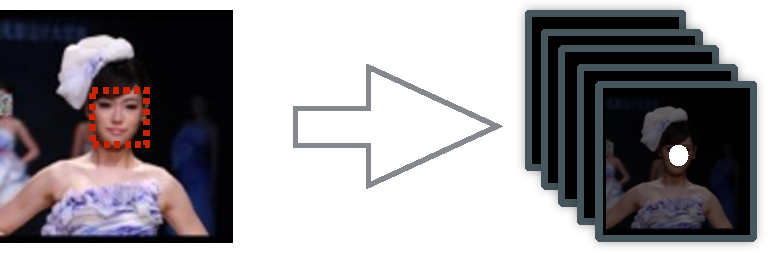
\includegraphics[scale=0.55]{figures/figure2-crop.pdf}
	\caption{\textbf{The Ground Truth Map in Training .} The left image is the input patch, and the right one is its ground truth map. }
	\label{fig:fig_gt}
	\end{figure}

Note that if multiple faces occur in one patch, we keep those faces as positive if they fall in a scale range(e.g. 0.8 to 1.25 in our setting) relative to the face in patch center. Other faces are treated as negative samples. The pixels of first channel, which denote the confidence score of class, in the ground truth map are initialized with 0, and further set to 1 if within the positive label region.  We also find our ground truth generation is quite similar to the segmentation work\cite{pinheiro2015learning} by Pinheiro et.al.   In their method, the pixel label is decided by the location of object in patch, while in DenseBox, the pixel label is determined by the receptive field. Specifically, if the output pixel is labeled to 1 if it satisfies the constraint that its receptive field contains an object roughly in the center and in a given scale. Each pixel can be treated as one sample , since every 5-channel pixel describe a bounding box.


\subsection{Model Design } 

Our network architecture illustrated in Fig \ref{fig:fig_net} is derived from the VGG 19 model used for image classification\cite{simonyan2014very}. The whole network has 16 convolution layers, with the first 12 convolution layers initialized by VGG 19 model.  The output of conv4\_4 is feed into four $1 \times 1$ convolution layers, where the first two convolution layers output 1-channel map for class score, and the second two predict the relative position of bounding box by 4-channel map.  The last $1 \times 1$ convolution layers act as fully connected layers in a sliding-window fashion.  


	\begin{figure}[!hbtp]
	\centering
	 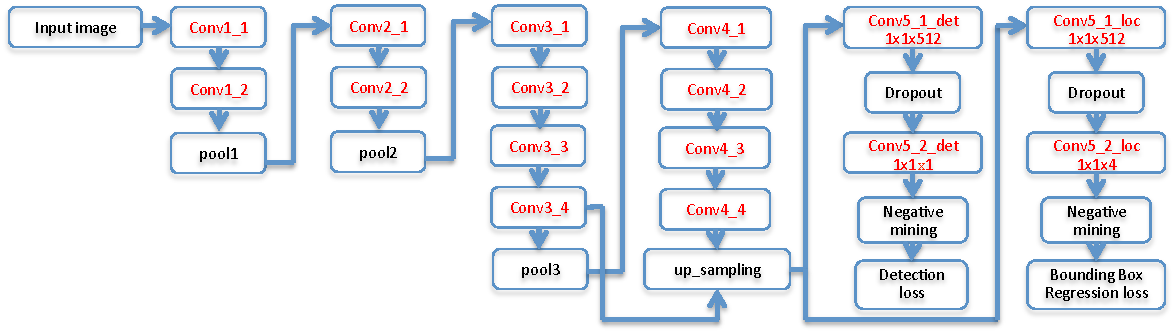
\includegraphics[scale=0.55]{figures/figure3-crop.pdf}
	\caption{\textbf{Network architecture of DenseBox.} The rectangles with red names contain learnable parameters. }
	\label{fig:fig_net}
	\end{figure}



\textbf{Multi-Level Feature Fusion.} 
Recent works\cite{bertasius2014deepedge, liu2015parsenet} indicate that using features from different convolution layers can enhance performance in task such as edge detection and segmentation. Part-level feature focus on local details of object to find discriminative appearance parts, while object-level or high-level feature usually has a larger receptive field in order to recognize object. The larger receptive field also brings in context information to predict more accurate result. In our implementation, we concatenate feature map from conv3\_4 and conv4\_4. The receptive field (or sliding window size) of conv3\_4 is $48 \times 48$, almost the same size of the face size in training, and the conv4\_4 have a much larger receptive field, around $118 \times 118$ in size, which could utilize global textures and context for detection.  Note that the feature map size of conv4\_4 is half of the map generated by conv3\_4, hence we use a bilinear up-sampling layer to transform them to the same resolution. 

\subsection{Multi-Task Training.} 
\label{sec:training} 
We use the ImageNet pre-trained VGG 19 network to initialize DenseBox. Actually, in initialization, we only keep the first 12 convolution layers(from conv1\_1 to conv4\_4), and the other layers in VGG 19 are replaced by four new convolution layers with “xavier” initialization. 

Like Fast R-CNN, our network has two sibling output branches.  The first outputs the confidence score $ \hat{y}$ (per pixel in the output map) of being a target object.  Given the ground truth label $y^* \in \{0,1 \}$ , the classification loss can be defined as follows. 
	\begin{equation}\label{eq:eq_cls_loss}
	\mathcal{L} _{cls}(\hat{y},y^*) = \left \| \hat{y} - y^* \right \| ^2
	\end{equation}
Here we use $L2$ loss in both face and car detection task. We did not try other loss functions such as hinge loss or cross-entropy loss, which seems to be a more appropriate choice, as we find the simple $L2$ loss work well in our task. 

The second branch of outputs the bounding-box regression loss, denoted as $\mathcal{L} _{loc}$.  It targets on minimizing the $L2$ loss between the predicted location offsets $\hat{d} = (\hat{d}_{tx}, \hat{d}_{ty}, \hat{d}_{tx}, \hat{d}_{ty})$ and the targets  $\ d^* = (d^{*}_{tx},  d^{*}_{ty},  d^{*}_{tx}, d^{*}_{ty})$, as formulized by:
	\begin{equation}\label{eq:eq_loc_loss}
	\mathcal{L} _{loc}(\hat{d},d^*) =  \sum_{i \in \{ tx, ty,bx,by \} }  \left \| \hat{d}_{i} - d^*_{i} \right \| ^2
	\end{equation}

 \subsubsection{Balance Sampling.} 
The process of selecting negative samples is one of the crucial parts in learning. If simply using all negative samples in a mini-batch will bias prediction towards negative samples as they dominate in all samples.  In addition, the detector will degrade if we penalize loss on those samples lying in the margin of positive and negative region.  Here we use a binary mask for each output pixel to indicate whether it is selected in training. 

\textbf{Ignoring Gray Zone.} 
The gray zone is defined on the margin of positive and negative region. It should not be considered to be positive or negative, and its loss weight should be set to $0$.  For each non-positive labeled pixel in the output coordinate space, its ignore flag $f_{ign}$ is set to 1 only if there is any pixel with positive label within $r_{near} = 2$ pixel length.  

\textbf{Hard Negative Mining.} 
Analogous to hard-negative mining procedure in SVM, we make learning more efficient by searching the badly predicted samples rather than random samples. After negative mining, the badly predicted samples are very likely to be selected, so that gradient descent learning on those samples leads more robust prediction with less noise. Specifically, negative mining can be performed efficiently by online bootstrap. In the forward propagation phase, we sort the loss (Eq \ref{eq:eq_cls_loss}) of output pixels in decending order, and assign the top 1\% to be hard-negative.   In all experiments, we keep all positive labeled pixels(samples) and the ratio of positive and negative to be 1:1.  Among all negative samples, half of them are sampled from hard-negative samples, and the remaining half are selected randomly from non-hard negative. For convenience, we set a flag $f_{sel} = 1$ to those pixels (samples) selected in a mini-batch. 

\textbf{Loss with Mask.} 
Now we can define the mask $M(\hat{t}_i)$ for each sample $\hat{t}_i = \{ \hat{y}_i, \hat{d}_i \}$ as a function of flags mentioned above:
	\begin{eqnarray}\label{eq:eq_mask}
	M(\hat{t}_i) =
	\begin{cases}
	0 &  f_{ign}^{i} = 1 \text{ or } f_{sel}^{i} = 0 \\
	1 & \text{otherwise} \\
	\end{cases}
	\end{eqnarray}
 Then if we combine the classification (Eq \ref{eq:eq_cls_loss})  and bounding box regression (Eq \ref{eq:eq_loc_loss}) loss with masks, our full multi-task loss can be represented as ,
	\begin{equation}\label{eq:eq_det_loss}
	\mathcal{L} _{det}(\theta) =  \sum_{i}  \left ( M(\hat{t}_i) \mathcal{L} _{cls}(\hat{y}_i,y^*_i) + \lambda_{loc} [y^*_i >0]M(\hat{t}_i) \mathcal{L} _{loc}(\hat{d}_i,d^*_i) \right )
	\end{equation}
where $\theta$ is the set of parameters in the network, and the Iverson bracket function $[y^*_i >0]$ is activated only if the ground truth score $y^*_i$ is positive. It is obvious that the bounding box regression loss should be ignored for negative samples (background), since there is no notation for them. The balance between classification and regression tasks is controlled by the parameter $\lambda_{loc}$. In our experiments, we normalize the regression target $d^*$ by dividing by the standard object height, which is $50/4$ in ground truth map, and $\lambda_{loc} = 3$ works well in all experiments under this normalization. 

\textbf{Other Implementation Details.} 
In training, an input patch is considered to be ``positive patch" if it contains an object centered in the center at a specific scale.  These patches only contain negative samples around the positive samples.  To fully explore the negative samples in the whole dataset, we also randomly crop patches at random scale from training images, and resize them to the same size and feed them to the network. We call this kind of patch as ``random patch", and the ratio of ``positive patch" and ``random patch" in training is 1:1.  In addition, to further increase the robustness of our model, we also randomly jitter every patch before feeding them into the network.  Specifically, we apply left-right flip, translation shift (of 25 pixels), and scale deformation (from $[0.8 , 1.25]$). 

We use mini-batch SGD in training and the batch size is set to 10. The loss and output gradients must be scaled by the number of contributing pixels, so that both loss and output gradients are comparable in multi-task learning. The global learning rate starts with 0.001, and it is reduced by a factor of 10 at every 100K iterations. We follow the default momentum term weight 0.9 and the weight decay factor 0.0005. 


\subsection{Refine with Landmark Localization.} 
	\begin{figure}[!hbtp]
	\centering
	 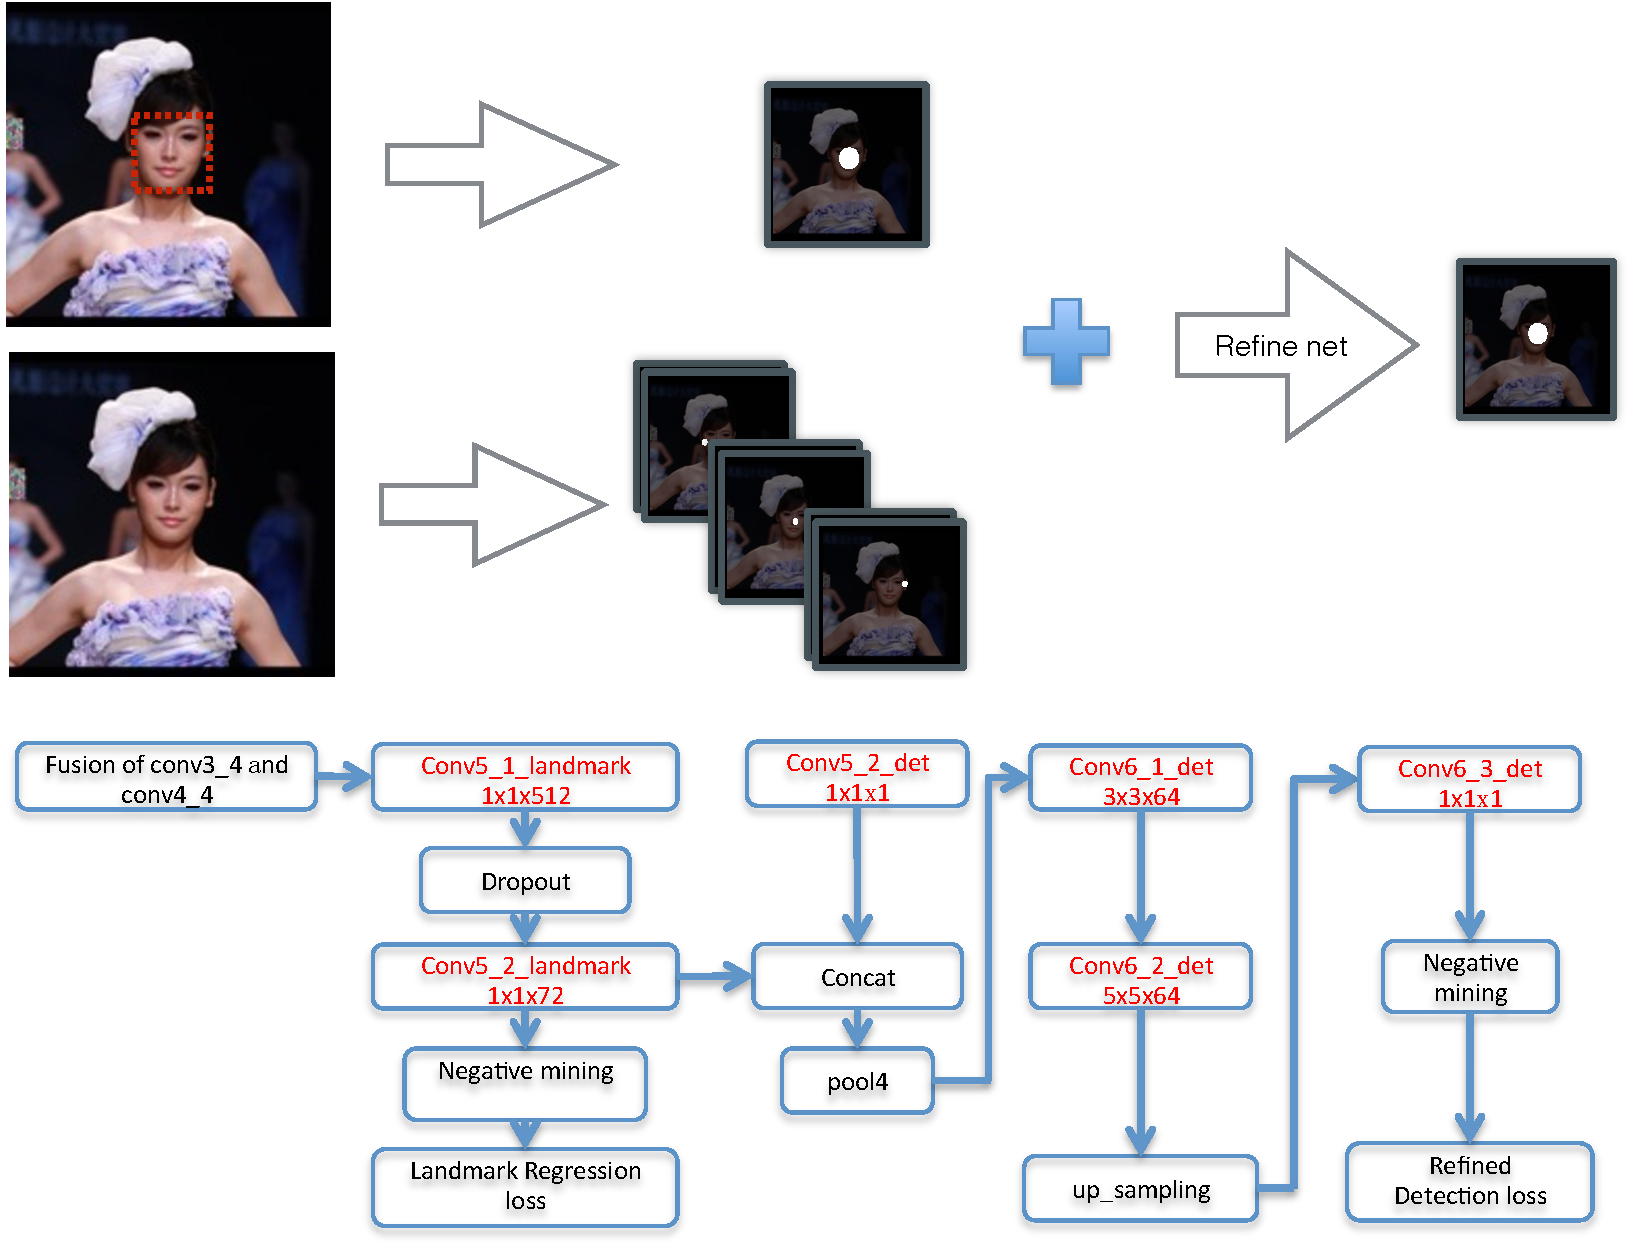
\includegraphics[scale=0.45]{figures/figure4-crop.pdf}
	\caption{\textbf{Top: } The pipeline of DenseBox with landmark localization. \textbf{Bottom: } The network structure for landmark localization. }
	\label{fig:fig_refine}
	\end{figure}
In this part, we show that landmark localization can be achieved in DenseBox just by stacking a few layers owe to the fully convolution architecture. Moreover, we can refine detection results through the fusion of landmark heatmaps and face score map. As shown in Fig \ref{fig:fig_refine},  we incorporate another sibling branch output for landmark localization. Suppose there are $N$ landmarks, the landmark localization branch outputs N response maps, with each pixel represent the confidence score of being a landmark at that location.  The appearance of ground-truth maps used for this task is quite similar to the ground-truth for detection.  For a landmark instance $l^k_i$, the $i$th instance of landmark $k$, its ground-truth is a positive labeled region located at the corresponding location on the $k$th response map in the output coordinate space.  Note that the radius $r_l$ should be relative small (e.g. $r_l = 1$  )to prevent loss of accuracy.   Similar to classification task, the landmark localization loss $\mathcal{L} _{lm}$is defined as a $L2$ loss between predicted values and labels, and we still apply the negative mining and ignore region discussed in the previous section. 

The final output refine branch, taking the classification score map and landmark localization maps as input, targets on refine of the detection results.  An appropriate solution could be using high-level spatial model to learn the constraints of landmark confidence and bounding box score, to further increase the performance of detections. Tompson et.al.\cite{tompson2014joint} proposed a MRF-like model using modified convolution (SoftPlus convolution) with non-negative output to connect the distribution of spatial location for each body part.  However, their model also include $Log$ and $Exp$ stages, which make model difficult to train.  In our implementation, we use convolutions with ReLU activation to approximate the spatial model.  If we denote the refine detection loss as $\mathcal{L} _{rf}$, which is almost the same as the classification loss $\mathcal{L} _{cls}$ mentioned before but the predict map is from the refine branch, the full loss becomes as ,
	\begin{equation}\label{eq:eq_full_loss}
	\mathcal{L} _{full}(\theta) = \lambda_{det} \mathcal{L} _{det}(\theta) + \lambda_{lm} \mathcal{L} _{lm}(\theta) + \mathcal{L} _{rf}(\theta)
	\end{equation}
where $\lambda_{det}$ and $\lambda_{lm}$ controll the balance of the three tasks. They are assigned to 1 and 0.5 respectively in our experiments. 

\subsection{Comparison } 
The highlight of DenseBox is that it frames object detection as a regression problem and provides an end-to-end detection framework.  Several recent works such as YOLO and Faster R-CNN have jointed region proposal generation with classifier together. Here we compare DenseBox to other related detection systems, pointing out the key similarities and differences. 
 
\textbf{Traditional NN-based Face Detector.} The neural network-based face detectors refer to those face detection system using neural network before the recent break-through results of CNNs for image classification. Applying neural networks for face detection has a long history, and the early works date back to 1990s\cite{vaillant1994original}.  Rowley et al.\cite{rowley1998neural} train neural network-based detectors which only is activated on faces with specific size, and apply detectors on the image pyramid with sliding-window fashion. Our DenseBox is very similar to them in the detection pipeline, excepting that we use modern CNNs as detectors. Hence the DenseBox could be called as `` Modern NN-based detector“ in one sense. 

\textbf{OverFeat.} OverFeat\cite{sermanet2013overfeat} designed by Sermanet et al. might be the first work that train a convolution neural network to perform classification and localization together after the success application of deep CNNs for image classification\cite{krizhevsky2012imagenet}. It also apply fully convolutional network on test time, an equivalent but much efficient way to perform sliding window detection. However it still disjoints classification and localization in training, and need complex post-processing to produce detection results. Our method is very similar to OverFeat but a multi-task jointly learned end-to-end detection network. 

\textbf{Deep Dense Face Detector (DDFD)} The DDFD, psoposed by Farfade et.al.\cite{farfade2015multi},  is a face detection system based on convolutional neural networks. It claims to have superior performance over R-CNN on face detection task due to the reason that proposal generation in R-CNN may miss some face regions.  Although the DDFD is a complete detection pipeline,  the DDFD is not an end-to-end framework since it separate the class probability prediction and bounding box localization as two tasks and two stages.  Our DenseBox can be optimized directly for detection , and can be easily improved by incorporating landmark information. 

\textbf{Faster R-CNN.} The faster R-CNN\cite{ren2015faster} still use region proposals to find objects in an image. Unlike the its former variants, the region proposals in faster R-CNN is produced by region proposal networks(RPNs) sharing convolutional feature computation with classifiers in the second stage. The PRN shares many similarities with our method DenseBox. However, The PRN needs predefined anchors while ours does not. The PRN is trained on multi-scale objects while the DenseBox presented in this paper is trained on one scale with jitter-augmentation, which means our method need to evaluate feature at multiple scales. Moreover, the training schemes are quite different between DenseBox and PRN. 

\textbf{MultiBox.} The MultiBox\cite{erhan2014scalable} trains a convolutional neural network to generate proposals instead of selective search. Both DenseBox and MultiBox are trained to predict bounding boxes in an image, they generate bounding boxes in different way.  As compared in \cite{ren2015faster} , the MultiBox method generates 800 non-translation-invariant anchors, whereas our DenseBox output translation-invariant bounding boxes like RPN. As the down-sampling factor of output map is 4,  DenseBox will densely generate one bounding box with score at every 4 pixels. 

\textbf{YOLO.}  Redmon et al.\cite{YOLO} propose a unified object detection pipeline, called YOLO. Both DenseBox and YOLO can be trained end-to-end from images, but the model design differs in the output layers.  The YOLO system takes a $448 \times 448$ image as input, and outputs $7 \times 7$ grid cells, only 49 bounding boxes per image. Our DenseBox uses up-sampling layers to keep a relative high-resolution output, with a down-sampling scale factor of 4 in our model. This enables our network capable to detect very small objects and highly overlapped objects, which YOLO is unable to deal with. 
 

